\documentclass[t]{beamer}

\usepackage[utf8]{inputenc}
\usepackage{latexsym}
\usepackage{amsmath}
\usepackage{amssymb}
\usepackage{amsthm}
\usepackage{graphicx}
\usepackage{caption}
\usepackage{subcaption}
\usepackage{hyperref}
\usepackage{tikz}

\usetheme{Pittsburgh}
\usecolortheme{spruce}
\setbeamertemplate{navigation symbols}{}
\logo{
\includegraphics[height=0.5cm]{aops-logo.png}}

%% \setlength{\parindent}{2ex}

\title{The Wonderful World of Pell's Equations}
\author{Dave Neary}
\date{January 2023}

\begin{document}

\frame{\titlepage}

\begin{frame}
	\frametitle{Outline}
	\tableofcontents
\end{frame}

\section{A number puzzle}

\begin{frame}
	\frametitle{Triangular square numbers}
\begin{figure}
  \centering
  \begin{subfigure}{.4\textwidth}
    \centering
    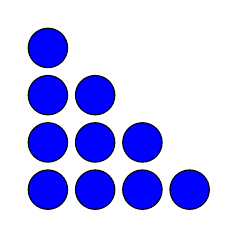
\begin{tikzpicture}
	\fill [blue,draw=black] (0,0) circle(0.25cm);
	\fill [blue,draw=black] (0,-0.6) circle(0.25cm) (0.6,-0.6) circle(0.25cm);
	\fill [blue,draw=black] (0,-1.2) circle(0.25cm) (0.6,-1.2) circle(0.25cm) (1.2,-1.2) circle(0.25cm);
	\fill [blue,draw=black] (0,-1.8) circle(0.25cm) (0.6,-1.8) circle(0.25cm) (1.2,-1.8) circle(0.25cm) (1.8,-1.8) circle(0.25cm);
    \end{tikzpicture}
    \caption*{Triangular numbers}
    \label{fig:triangular}
  \end{subfigure}
  \begin{subfigure}{.4\textwidth}
    \centering
    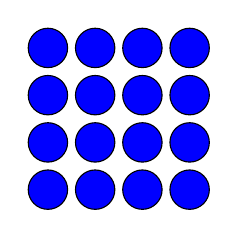
\begin{tikzpicture}
	\fill [blue,draw=black] (0,0) circle(0.25cm) (0.6,0) circle(0.25cm) (1.2,0) circle(0.25cm) (1.8,0) circle(0.25cm);
	\fill [blue,draw=black] (0,-0.6) circle(0.25cm) (0.6,-0.6) circle(0.25cm) circle(0.25cm) (1.2,-0.6) circle(0.25cm) (1.8,-0.6) circle(0.25cm);
	\fill [blue,draw=black] (0,-1.2) circle(0.25cm) (0.6,-1.2) circle(0.25cm) (1.2,-1.2) circle(0.25cm) circle(0.25cm) (1.8,-1.2) circle(0.25cm);
	\fill [blue,draw=black] (0,-1.8) circle(0.25cm) (0.6,-1.8) circle(0.25cm) (1.2,-1.8) circle(0.25cm) (1.8,-1.8) circle(0.25cm) circle(0.25cm);
    \end{tikzpicture}
    \caption*{Square numbers}
    \label{fig:squares}
  \end{subfigure}
\end{figure}

	Can you find triangular numbers (of the form $1+2+3+\cdots+n$) that are also perfect squares ($m^2$ for an integer $m$)?	
\end{frame}

\begin{frame}
  \frametitle{Triangular numbers}
  Can we find a formula for the $n$th triangular number:
  \[T_n = 1+2+3+\cdots + a \]

\end{frame}

\begin{frame}
        \frametitle{Triangular Square numbers}
	We are looking for solutions to:
	\begin{align*}
		\frac{1}{2}(a)(a+1) &= b^2 \\
		a^2 + a &= 2b^2 \\
		4a^2 + 4a &= 8b^2 \\
		(2a+1)^2 - 8b^2 &= 1
	\end{align*}
	Setting $m=2a+1, n=2b$, we get the Pell's equation:
	\[ m^2 - 2n^2 = 1 \]
\end{frame}

\begin{frame}
        \frametitle{Pell's Equations: $m^2 - dn^2 = 1$}
	\[ m^2 - dn^2 = 1 \]

	Equations of this form are called Pell's equations after John Pell, who
	translated a text on the equation into English, and Euler thought it was
	original work, and named the equation after him.

	\vspace{1em}Equations of this form have been studied for centuries (especially by
	Indian mathematicians Brahmagupta and Bh\=askara II).

	\vspace{1em}Geometrically, the curve is a hyperbola, but tonight, we will 
	explore its connections to number theory.
\end{frame}


\begin{frame}
	\frametitle{Finding solutions}

	By inspection, we can find $m=3, n=2$ works:
	\[ 3^2 - 2(2^2) = 9 - 8 = 1 \]
	But can we find other solutions?\\
	It's a bit trickier!

	\vspace{2em}

	What does $m^2 - 2n^2$ remind you of?
\end{frame}

\begin{frame}
	\frametitle{Factoring as a difference of squares}

	\[ m^2 - 2n^2 = (m-\sqrt{2}n)(m+\sqrt{2}n) \]

	But now if we have two numbers of the form $m^2-2n^2$ what happens
	when we multiply these factors?

	\begin{align*}
		(a-\sqrt{2}b)(c-\sqrt{2}d) &= ac - \sqrt{2}bc - \sqrt{2}ad + 2bd \\
		&= (ac+2bd)-\sqrt{2}(bc+ad)
	\end{align*}

	\begin{align*}
		(a+\sqrt{2}b)(c+\sqrt{2}d) &= ac + \sqrt{2}bc + \sqrt{2}ad + 2bd \\
		&= (ac+2bd)-\sqrt{2}(bc+ad)
	\end{align*}


\end{frame}

\begin{frame}
	\frametitle{Numbers $a+\sqrt{2}b$ are closed under multiplication}

	This means is that when we multiply numbers of the form $a+\sqrt{2}b$ 
	together, they give a result of the same form!

	\vspace{1em}
	These numbers are an extension to the integers - we can add, subtract,
	and multiply numbers $a+\sqrt{2}b$ together and the result is in the
	same form.

	\vspace{1em}
	What's more: 
	\[(a-\sqrt{2}b)(c-\sqrt{2}d) = A-\sqrt{2}B \]
	\[(a+\sqrt{2}b)(c+\sqrt{2}d) = A+\sqrt{2}B \]

\end{frame}

\begin{frame}
	\frametitle{Generating larger solutions}
	What this means is that when we multiply numbers of the form $a^2-2b^2$,
	we can make the product into the form $A^2 - 2B^2$ for some integers $A,B$.

	But we can now generate larger solutions to our problem!

	\[ (3-2\sqrt{2})^2(3+2\sqrt{2})^2 = (17 - 12\sqrt{2})(17 + 12\sqrt{2}) = 1^2 \]

	\[ (3-2\sqrt{2})^3(3+2\sqrt{2})^3 = (99 - 70\sqrt{2})(99 + 70\sqrt{2}) = 1^3 \]

	There are an infinite number of solutions!
\end{frame}


\section{Approximating square roots}

\begin{frame}
        \frametitle{Notice anything?}
	\[3^2 - 2(2^2) = 1, \frac{3}{2} = 1.5 \]
	\[17^2 - 2(12^2) = 1, \frac{17}{12} = 1.41666\cdots \]
	\[99^2 - 2(70^2) = 1, \frac{99}{70} = 1.414285\cdots \]

	These numbers are getting close to a well known constant... why?
\end{frame}

\begin{frame}
	\frametitle{Approximating $\sqrt{2}$}

	If we take large solutions to:
	\[ a^2 - 2b^2 = 1 \]

	then:
	\[ \left(\frac{a}{b}\right)^2 = 2 + \frac{1}{b^2} \]

	and as $b$ gets large, $\frac{a}{b}$ gets very close to $\sqrt{2}$.

	\vspace{1em}
	Bonus trick: if one estimate is $\frac{a}{b}$, can you prove that the 
	next one is $\frac{3a+4b}{2a+3b}$ and explain why?
\end{frame}

\begin{frame}
        \frametitle{Choosing a different value for $d$}

	This works just as well for other values of $d$. For example,
	with $d=5$:

	\[ m^2 - 5n^2 = 1 \]

	has a solution at $a=9,b=4$: $9^2 - 5(4^2) = 1$.

	We can get very good estimates for $\sqrt{5}$ by raising this solution 
	to different powers:
	\[ (9-4\sqrt{5})^2 = 161 - 72\sqrt{5} \]
	\[ \frac{161}{72} = 2.2361\cdots, \sqrt{5} = 2.23606\cdots \]
\end{frame}

\section{Finding smallest solutions for $m^2-dn^2=1$}

\begin{frame}
        \frametitle{Finding the smallest solution}

	Finding $a=9,b=4$ for $d=5$ was a little trickier than for $d=2$ - in
	general, how can we find the smallest solution without checking every number?

	\vspace{1em}
	For example: what is the smallest solution for $d=10$? Or $d=13$?
\end{frame}

\begin{frame}
	\frametitle{Continuous fractions!}

	Enter continued fractions! Any positive real number can be expressed as a
	continuous fraction of the form:

	\[ x = a_0 + \frac{1}{a_1 + \frac{1}{a_2+\frac{1}{a_3+\cdots}}} \]

	where every one of the $\{a_i\}$ are whole numbers.

	\vspace{1em}
	When written like this, we can find good rational approximations to the
	number $x$ by stopping the calculation after a few numbers. These
	approximations are called "convergents".
\end{frame}

\begin{frame}
	\frametitle{Calculating a continued fraction for $\sqrt{10}$}

	Since $3 < \sqrt{10} < 4$:

	\[ \sqrt{10} = 3 + (\sqrt{10} - 3) \]

\end{frame}

\begin{frame}
	\frametitle{Calculating the convergents for $\sqrt{10}$}

	We found on the last slide that:

	\[ \sqrt{10} = 3 + \frac{1}{6 + \frac{1}{6 + \frac{1}{6 + \cdots}}} \]
	
	We can now calculate the first few convergents:

	\[ 3 + \frac{1}{6} = \frac{19}{6} \]
	\[ 19^2 - 10(6^2) = 361 - 10(36) = 1 \]

	And we have our smallest solution!

\end{frame}

\begin{frame}
	\frametitle{Complicated solutions}
	
	There are some famously difficult first solutions, for example: $d = 13$
	\[ \sqrt{13} = 3 + \frac{1}{1+\frac{1}{1+\frac{1}{1+\frac{1}{1+\frac{1}{6+\cdots}}}}}\]

	The convergents for this continued fraction are:
	\[ \frac{3}{1}, \frac{4}{1}, \frac{7}{2}, \frac{11}{3}, \frac{18}{5}, \frac{119}{33}, \frac{137}{38}, \frac{256}{71}, \frac{393}{109}, \frac{649}{180}, \cdots \]

	The smallest solution to $m^2-13n^2=1$ is
	\[ 649^2 - 13(180^2) = 1 \]

	Challenge: Can you find the smallest solution to $m^2-41n^2=1$?

\end{frame}

\begin{frame}
	\frametitle{Conclusion}

	The Pell's equations pull together diverse fields of mathematics:
	
	\vspace{1em}
	\begin{itemize}
		\item Number theory - extensions to the integers
		\item Rational approximations for irrational numbers
		\item Continued fractions
		\item Algebraic geometry
	\end{itemize}

	\vspace{1em}
	These equations continue to be relevant today! 

\end{frame}

\end{document}
